\graphicspath{{images/}}

\subsection{Численные методы решения ДУЧП эллиптического типа}

\subsubsection{Постановка задачи}
Решить краевую задачу для дифференциального уравнения эллиптического типа. Аппроксимацию уравнения произвести с использованием центрально-разностной схемы. Для решения дискретного аналога применить следующие методы: метод простых итераций (метод Либмана), метод Зейделя, метод простых итераций с верхней релаксацией. Вычислить погрешность численного решения путем сравнения результатов с приведенным в задании аналитическим решением $U(x,y)$.  Исследовать зависимость погрешности от сеточных параметров $h_x$, $h_y$.

\subsubsection{Вариант 8}
$$ {{\partial^2 u} \over {\partial x^2}} + {{\partial^2 u} \over {\partial y^2}} = -2\cdot{{\partial u} \over {\partial x}} -3 \cdot u $$
$$ u(0, y) = \cos{y} $$
$$ u({{\pi} \over {2}}, y) = 0 $$
$$ u(x, 0) = e ^ {-x} \cdot \cos{x} $$
$$ u(x, {{\pi} \over {2}}) = 0 $$
Аналитическое решение:
$$ U(x, y) = e ^ {-x} \cdot \cos{x} \cdot \cos{y} $$
\pagebreak

\subsubsection{Результат}
\begin{center}
    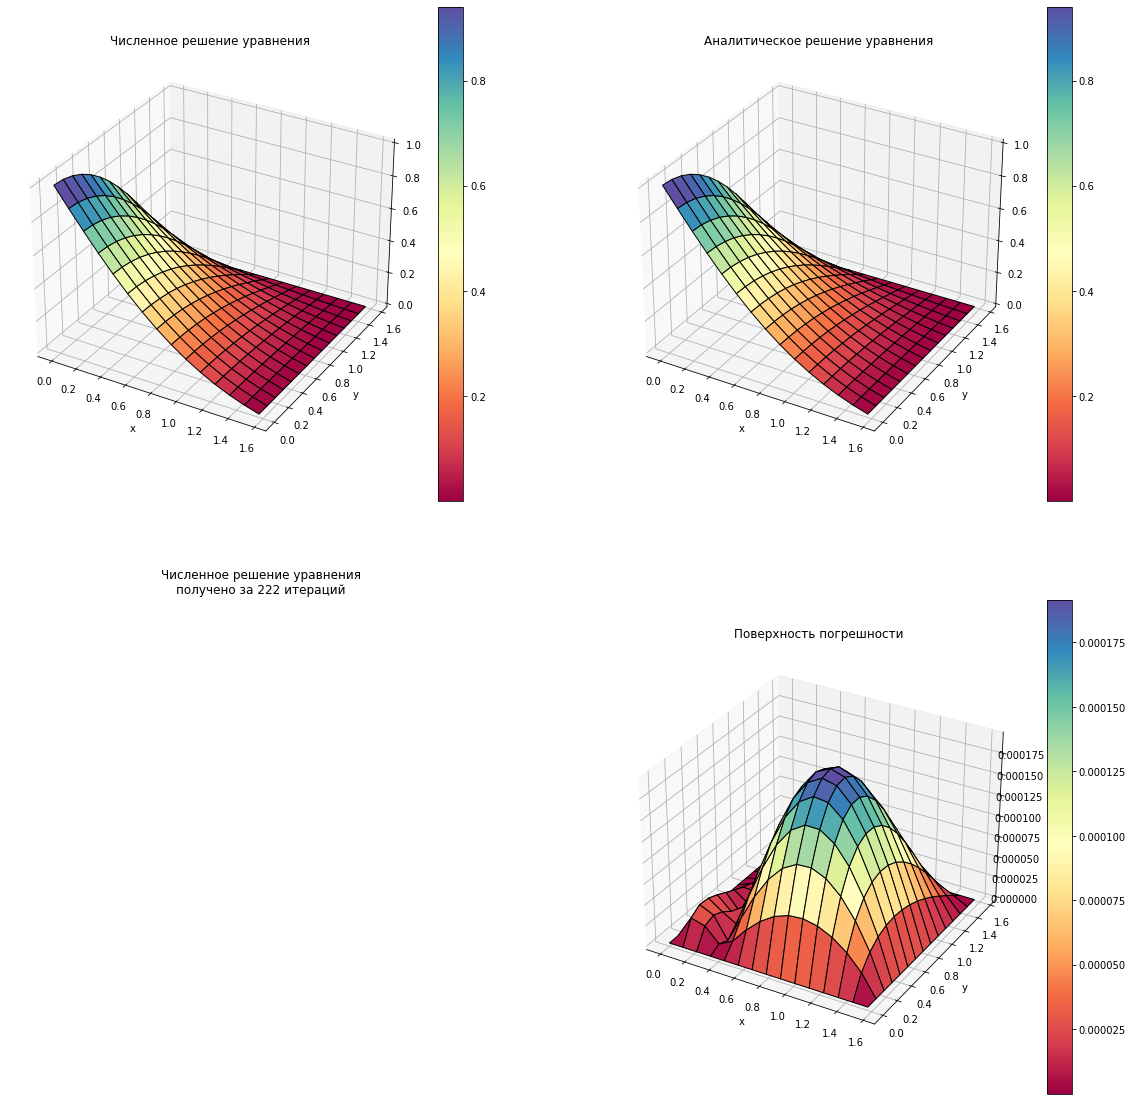
\includegraphics[width=\textwidth]{7.png}\newline\noindent
\end{center}
\pagebreak

\subsubsection{Исходный код}
\lstinputlisting{../lab7/epde.hpp}
\pagebreak
